\documentclass[a4paper]{article}
\usepackage[utf8]{inputenc}
\usepackage[spanish, es-tabla]{babel}

\usepackage{amsmath}
\usepackage{amsfonts}
\usepackage{amssymb}

\usepackage{float}
\usepackage{graphicx}
\graphicspath{ {./Imagenes/} }

\usepackage[american voltage]{circuitikz}

\usepackage{fancyhdr}

\usepackage{units} 

\pagestyle{fancy}
\fancyhf{}
\lhead{22.02 Electrotecnia I}
\rhead{Mechoulam, Mestanza, Lambertucci, Pouthier, Londero}
\rfoot{Página \thepage}



\begin{document}

%%%%%%%%%%%%%%%%%%%%%%%%%%%%%%%%%%%%%%%%%%%%%%%%%%%%%%%%%%%%%%%%%%%%%%%%% 
%								CARATULA								%
%%%%%%%%%%%%%%%%%%%%%%%%%%%%%%%%%%%%%%%%%%%%%%%%%%%%%%%%%%%%%%%%%%%%%%%%% 

\begin{titlepage}
\newcommand{\HRule}{\rule{\linewidth}{0.5mm}}
\center
\mbox{\textsc{\LARGE \bfseries {Instituto Tecnológico de Buenos Aires}}}\\[1.5cm]
\textsc{\Large 22.02 Electrotecnia I}\\[0.5cm]


\HRule \\[0.6cm]
{ \Huge \bfseries Trabajo práctico N$^{\circ}$2}\\[0.4cm] 
\HRule \\[1.5cm]


{\large

\emph{Grupo 5}\\
\vspace{3px}

\begin{tabular}{lr} 	
\textsc{Mechoulam}, Alan  &  \\
\textsc{Lambertucci}, Guido Enrique  & 58009 \\
\textsc{Pouthier}, Florian  & 61337 \\
\textsc{Mestanza}, Nicolás  & 61337 \\
\textsc{Londero Bonaparte}, Tomás Guillermo  & 58150 \\
\end{tabular}

\vspace{20px}

\emph{Profesores}\\
\vspace{3px}
\textsc{Muñoz}, Claudio Marcelo\\ 	
\textsc{Ayub}, Gustavo\\ 	

\vspace{100px}

\begin{tabular}{ll}

Presentado: & 26/04/19\\

\end{tabular}

}

\vfill

\end{titlepage}


%%%%%%%%%%%%%%%%%%%%%%%%%%%%%%%%%%%%%%%%%%%%%%%%%%%%%%%%%%%%%%%%%%%%%%%%% 
%								INFORME									%
%%%%%%%%%%%%%%%%%%%%%%%%%%%%%%%%%%%%%%%%%%%%%%%%%%%%%%%%%%%%%%%%%%%%%%%%%

\section*{Introducción}
La experiencia realizada consistió en el análisis del período transitorio de diversos circuitos RC (desconocido) y RLC serie, variando los componentes de este último. Dentro de los elementos utilizados se encuentran:
	\begin{itemize}
	\item[$\bullet$]	Osciloscopio;
	\item[$\bullet$]	Multímetro;
	\item[$\bullet$]	Fuente de tensión;
	\item[$\bullet$]	Resistencia variable;
	\item[$\bullet$]	Banco de capacitores;
	\item[$\bullet$]	Inductor.
	\end{itemize}	  

\section*{Desarrollo de la experiencia}

\subsection*{\underline{Ejercicio 1}}

%%%%%%%%%%%%%%%%%%%%%%%%%%%%%%%%%%%%%%%%%%%%%%%%%%%%%%%%%%%%%%%%%%%%%%%%%
%		a. Determinar si es una configuración RC serie o RC paralelo.	%
%%%%%%%%%%%%%%%%%%%%%%%%%%%%%%%%%%%%%%%%%%%%%%%%%%%%%%%%%%%%%%%%%%%%%%%%%

En este primer ejercicio, se determinó la configuración de un circuito dispuesto en una caja, pudiendo ser RC serie o RC paralelo. Para hallarlo se decidió medir la continuidad entre la entrada y la salida de este. Una vez constatada, se midió, de la misma forma,  el valor de la resistencia del circuito, debido a que en caso de ser un circuito RC paralelo, el multímetro indicaría un valor fuera de escala, en caso contrario, se obtendría el valor de dicho dispositivo. De esta forma se concluyó que la forma del circuito es el que se muestra en la figura \ref{RCserie}, es decir, RC serie.

\begin{figure}[H]
\begin{center}
\begin{circuitikz}
	\draw
	(0,0) 	to (2.5,0)
		 	to [R, l=$R$] (4.5,0) 
			to (8,0)
			to [short, -o](9,0)
	(0,0)	to [V, l=$V_{1}$] (0,-3)
	(5.5,0)	to [C, l=$C$] (5.5,-3)
	(0,-3) 	to (8,-3) 
			to [short, -o](9,-3);
	\draw[dashed]
	(2,-4) to (2,1) to (7,1) to (7,-4) to (2,-4);
\end{circuitikz}
\end{center}

\caption{Circuito RC serie.} 
\label{RCserie}
\end{figure}

Mediante este razonamiento se pudo llegar a la conclusión de que el circuito es un RC serie, como se mostró anteriormente, es decir, la salida de dicho sistema se encuentra en paralelo con el capacitor.

%%%%%%%%%%%%%%%%%%%%%%%%%%%%%%%%%%%%%%%%%%%%%%%%%
%		b. Medir la respuesta transitoria.		%
%%%%%%%%%%%%%%%%%%%%%%%%%%%%%%%%%%%%%%%%%%%%%%%%%

Una vez establecido el tipo de circuito dispuesto, se prosiguió con el analisis de su respuesta transitoria. Se conectó el dispositivo a una fuente de tensión, se reguló la entrada a $ 5 V $ y mediante el uso de un osciloscopio se pudo observar la carga del capacitor.

\begin{figure}[H]
	\centering
	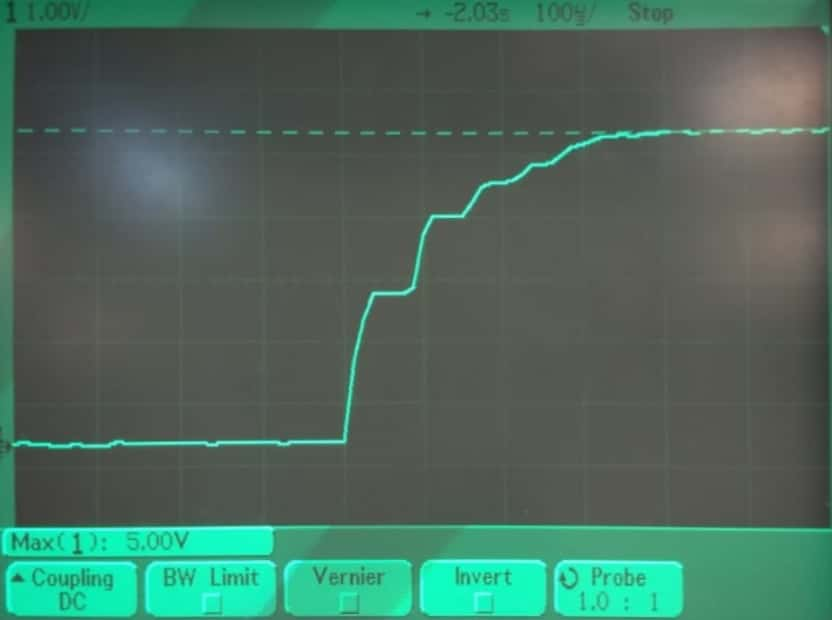
\includegraphics[width=0.8\textwidth]{Carga-transitoria-real.jpeg}
\caption{Voltaje medido a la salida del circuito al someterlo a $ 5\ V $.}
	\label{fig:carg-real}
\end{figure}

Por ultimo, de la misma forma, se pudo observar su descarga al retirar la tensión proporcionada.

\begin{figure}[H]
	\centering
	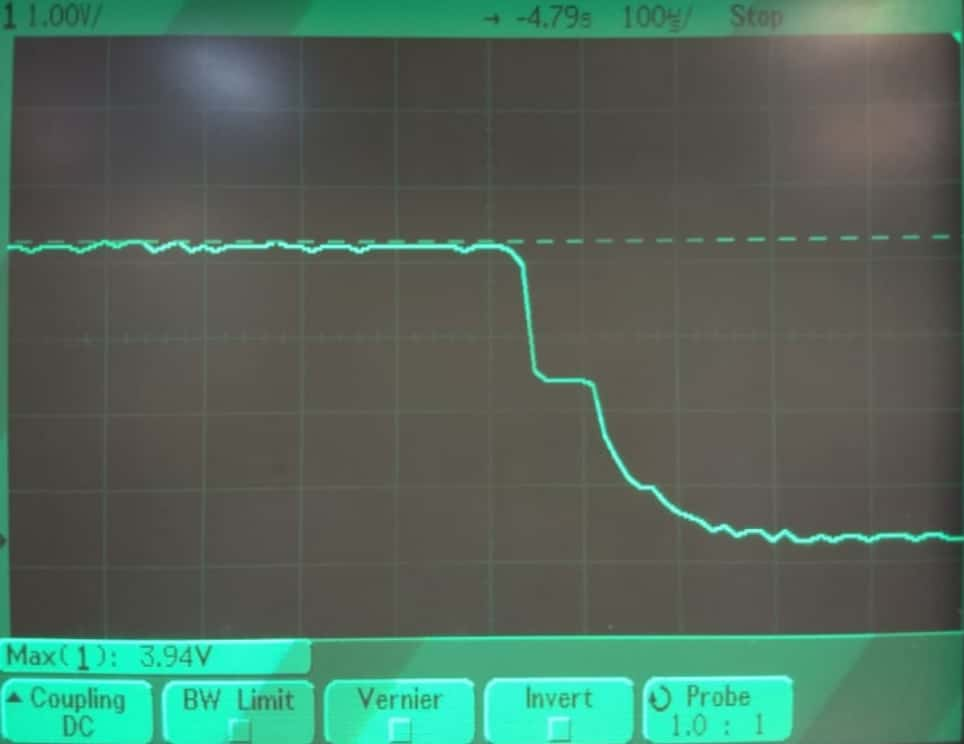
\includegraphics[width=0.8\textwidth]{Descarga-transitoria-real.jpeg}
	\caption{Voltaje medido a la salida del circuito al quitarle la alimentación.}
	\label{fig:desc-real}
\end{figure}

%%%%%%%%%%%%%%%%%%%%%%%%%%%%%%%%%%%%%%%%%%%%%%%%%%%%%%%%%%%%%%%%%
%		c. Medir la constante de tiempo del circuito.			%
%		d. obtener los valores de R y C experimentalmente.		%
%%%%%%%%%%%%%%%%%%%%%%%%%%%%%%%%%%%%%%%%%%%%%%%%%%%%%%%%%%%%%%%%%

Otro interés del trabajo fue hallar la constante de tiempo del circuito $ \tau = RC $. Para esto primero se obtuvo el valor de la resistencia $ R $ colocando un un multímetro a la entrada y salida del circuito, obteniéndose $ R_{exp} = 223.5 \Omega $.
Luego, sabiendo que la tensión en el capacitor al cargarse es

\begin{equation}
	V_{C} (t) = V_{f} \left( 1 - e^{- \frac{t}{RC}  } \right)
	\label{eq:carg-eq}
\end{equation}

y que $ V_{C} (\tau) = 0,63 V_{f} $, siendo $ V_{f} $ la tensión de la fuente, se observa de la figura \ref{fig:carg-real} el tiempo al que se llega a una tension de $ 3,15 V $, obteniendo así $ \tau = 90\ \mu s $. Por último, ya con el valor de la resistencia y del tiempo característico, se puede calcular el valor del capacitor, siendo este $ C = 0,40\ \mu f $.

%%%%%%%%%%%%%%%%%%%%%%%%%%%%%%%%%%%%%%%%%%%%%%%%%%%%%%%%%%%%%%%%%
%		e. Obtener la respuesta transitoria por simulación		%
%%%%%%%%%%%%%%%%%%%%%%%%%%%%%%%%%%%%%%%%%%%%%%%%%%%%%%%%%%%%%%%%%

Al tener los valores experimentales calculados, es posible modelar, de manera teórica, la carga y descarga del capacitor, mediante la ecuación \ref{eq:carg-eq} y la ecuación

\begin{equation}
	V_{C} (t) = V_{0} \ e^{-\frac{t}{RC}} 
	\label{eq:des-eq}
\end{equation}

siendo $ V_{0} $ la tensión inicial del capacitor, que en nuestro caso, es igual a la de la fuente, debido a que se puede considerar que este estuvo conectado mucho tiempo, alcanzando el régimen permanente.
Es así que se obtienen los siguientes gráficos:

\begin{figure}[H]
	\centering
	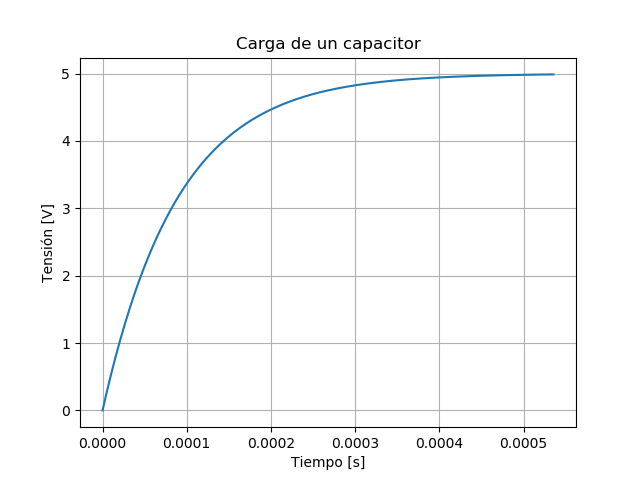
\includegraphics[width=0.8\textwidth]{Carga-transitoria-teorica.png}
\caption{Voltaje en función del tiempo a la salida del circuito con $ V_{0} = 0\ V $.}
	\label{fig:carg-teo}
\end{figure}

\begin{figure}[H]
	\centering
	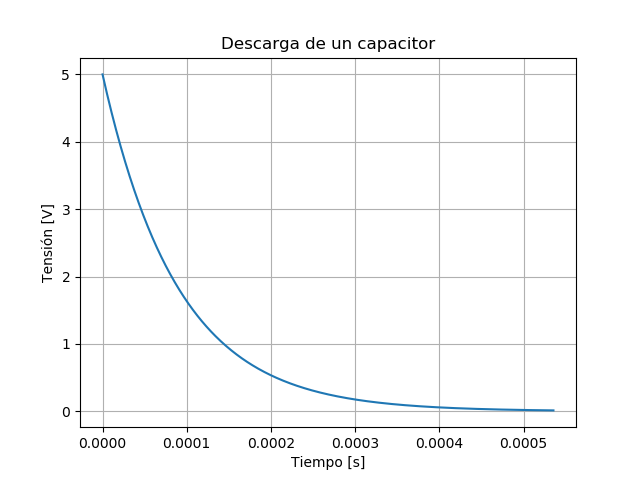
\includegraphics[width=0.8\textwidth]{Descarga-transitoria-teorica.png}
	\caption{Voltaje en función del tiempo a la salida del circuito con $ V_{0} = 5\ V $.}
	\label{fig:desc-teo}
\end{figure}

%%%%%%%%%%%%%%%%%%%%%%%%%%%%%%%%%%%%%%%%%%%%%%%%%%%%%%%%%%%%%%%%%%%%%%%%%%%%%%%%%
%		f. Representar gráficamente y comparar curvas b) y e) y conclusiones.	%
%%%%%%%%%%%%%%%%%%%%%%%%%%%%%%%%%%%%%%%%%%%%%%%%%%%%%%%%%%%%%%%%%%%%%%%%%%%%%%%%%

Al comparar las figuras \ref{fig:carg-real} con \ref{fig:carg-teo} y \ref{fig:desc-real} con \ref{fig:desc-teo}, se termina de confirmar que el circuito analizado es RC paralelo. Se observa que los gráficos teóricos corresponden a los brindados por el osciloscopio, salvando las diferencias de que, tanto la carga como la descarga teórica comienzan para un tiempo inicial nulo y que en estos últimos gráficos se observan los "saltos", atribuidos al ruido ajeno y al carácter no ideal que poseen los elementos utilizados.

\newpage

\subsection*{\underline{Ejercicio 2}}

\vspace{1em}
En el siguiente ejercicio se buscó visualizar el transitorio de la tensión del capacitor en un circuito RLC serie, luego puenteando la resistencia y finalmente con la inductancia. 

\begin{figure}[H]
	\centering
	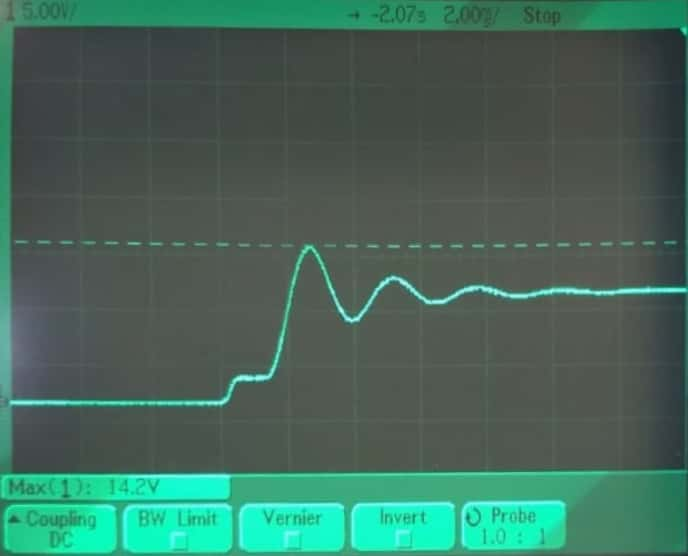
\includegraphics[width=0.8\textwidth]{carga-rlc.jpeg}
\caption{Tension sobre el Capacitor, RLC serie.}
	\label{fig:carg-rlc}
\end{figure}
\begin{figure}[H]
	\centering
	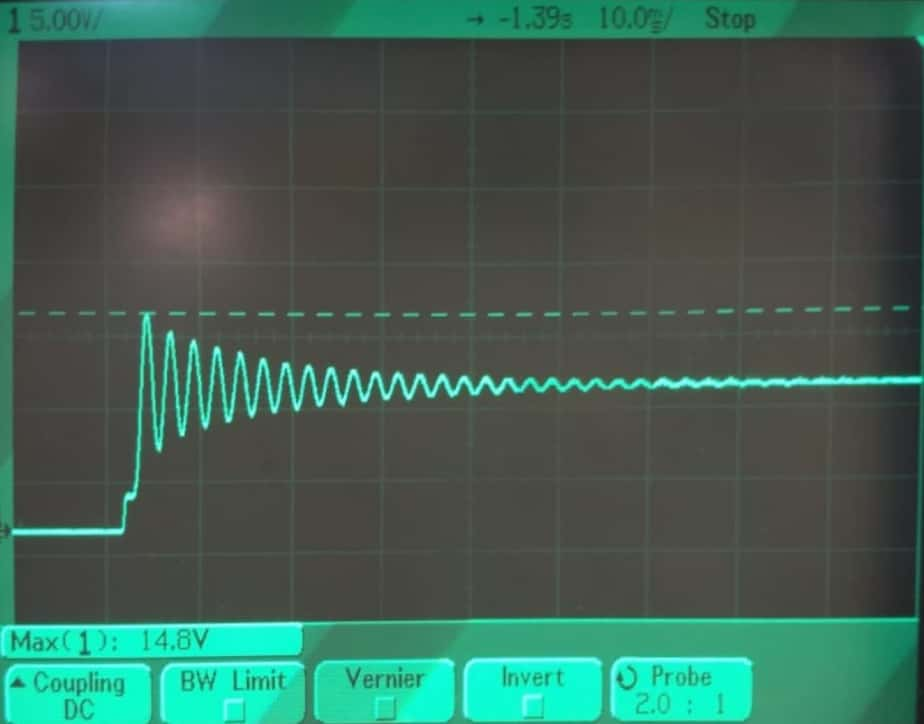
\includegraphics[width=0.8\textwidth]{carga-rlc-nor.jpeg}
\caption{Tension sobre el Capacitor, LC serie.}
	\label{fig:carg-lc}
\end{figure}
\begin{figure}[H]
	\centering
	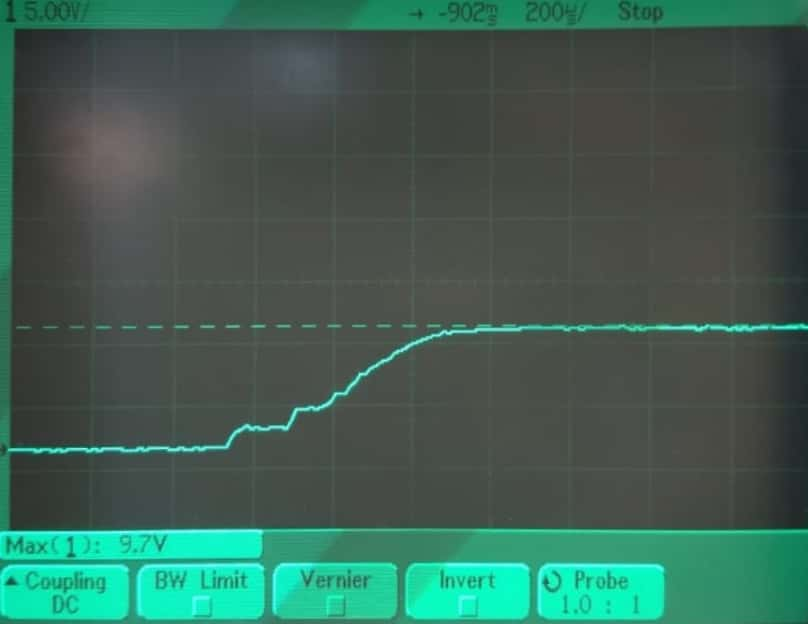
\includegraphics[width=0.8\textwidth]{carga-rlc-nol.jpeg}
\caption{Tension sobre el Capacitor, RC serie.}
	\label{fig:carg-rc}
\end{figure}



Se considera ahora el circuito RLC serie de la Figura \ref{RLCserie}.

\begin{figure}[H]
\begin{center}
\begin{circuitikz}
	\draw
	(0,0) 	to [V, l=$V_{2}$] (0,-3)
	(0,0) 	to (1,0) 
	(3,0)	to (2.5,0)
			to [spst] (2,0)
			to (1,0)
	(2,-3)	to (2,-0.5)
	(3,0)	to [L, l=$L$] (5,0)
			to [C, l=$C$] (7,0)
			to [R, l=$R$] (7,-3)
			to (0,-3);
\end{circuitikz}
\end{center}
\caption{Circuito RLC serie}
\label{RLCserie}
\end{figure}

Resolviendo este circuito usando el \textit{método de mallas}, se puede escribir:
\begin{equation}\label{mallas}
v_{2}(t) = v_{R}(t)+v_{L}(t)+v_{C}(t).
\end{equation}
Debido a que durante el experimetno no se obtuvieron los valores tanto de L y C se decidió obtener estos últimos basandose en las graficas del osciloscopio. Mirando la figura \ref{fig:carg-rlc} se puede observar el tiempo caracteristico en 0.63 Vmax se puede despejar el valor de L y midiendo la distancia entre periodos se puede obtener $\omega$'  y de alli con el valor de L despejar C 

%Sin embargo, sabemos que:
%\begin{equation}\label{vryvc}
%v_{R}=R \cdot i(t)
%\quad\text{y}\quad
%v_{L}=L\cdot\frac{di(t)}{dt}
%\end{equation}
%y también que la corriente en el circuito es dado por:
%\begin{equation}\label{corriente}
%i(t)=C \cdot \frac{dv_{C}(t)}{dt}
%\end{equation}
%
%Reemplazando por la expresión (\ref{corriente}) de la corriente en las expresiones de (\ref{vryvc}), se obtiene:
%\begin{equation}
%v_{R}(t)=RC\cdot\frac{dv_{C}(t)}{dt}
%\quad\text{y}\quad
%v_{L}(t)=LC\cdot\frac{d^{2}v_{C}(t)}{dt^{2}}.
%\end{equation}
%
%Entonces, la ecuación (\ref{mallas}) se escribe
%
%\begin{equation}
%LC\cdot\frac{d^{2}v_{C}(t)}{dt^{2}}+RC\cdot\frac{dv_{C}(t)}{dt}+v_{C}(t)=v_{2}(t),
%\end{equation}
%o también

Operando, se llega a la ecuación diferencial:
\begin{equation}
\frac{d^{2}v_{C}(t)}{dt^{2}}+\frac{R}{L}\cdot\frac{dv_{C}(t)}{dt}+\frac{1}{LC}\cdot v_{C}(t)=\frac{1}{LC}\cdot v_{2}(t).
\end{equation}

Considerando que $v_2 = 9.7\textrm{V}$, $R = 250\Omega$, $L = 250mHy$, $C = 900nF$ \[\Rightarrow \omega=\frac{1}{\sqrt{LC}}= 2108.185\quad y \quad \alpha=\frac{R}{2L}= 500\] \[\Rightarrow \omega > \alpha\] se puede observar que la solución será de carácter subamortiguado.\\

En el caso de que $R=0$, la ecuación del circuito se vuelve:
\begin{equation}
\frac{d^{2}v_{C}(t)}{dt^{2}}+\frac{1}{LC}\cdot v_{C}(t)=\frac{1}{LC}\cdot v_{2}(t).
\end{equation}

%La solución de esa ecuación diferencial se escribe:
%\begin{equation}
%v_{C}(t)=v_{Ch}(t)+v_{Cp}(t),
%\end{equation}
%donde :
%\begin{itemize}
%\item[$\bullet$] $v_{Cp}(t)$ es la \emph{solución particular} de la ecuación o modo forzado, dado por:
%\begin{equation}
%v_{Cp}(t)=V_{2}=v_{2}(t\to\infty)
%\end{equation}
%\item[$\bullet$] $v_{Ch}(t)$ es la \emph{solución homogéneo} de la ecuación, es decir la solución de la ecuación (\ref{eqHom}):
%\begin{equation}\label{eqHom}
%\frac{d^{2}v_{Ch}(t)}{dt^{2}}+\frac{1}{LC}\cdot v_{Ch}(t)=0
%\quad\Leftrightarrow\quad
%\frac{d^{2}v_{Ch}(t)}{dt^{2}}+\omega_{0}^{2}\cdot v_{Ch}(t)=0
%\end{equation}
%donde
%\begin{equation}
%\omega_{0}=\frac{1}{\sqrt{LC}}.
%\end{equation} 
%Considerando que $v_{Ch}(t)$ es de la forma $v_{Ch}(t)=e^{\beta t}$, se halla sustituando esa expresión en (\ref{eqHom}):
%\begin{equation}
%\beta^{2}e^{\beta t}+\omega_{0}^{2}e^{\beta t}=0
%\quad\Leftrightarrow\quad
%\beta^{2}+\omega_{0}^{2}=0
%\end{equation}
%\end{itemize}

%Para concluir, en el caso de $R_{t}=0$, se obtiene un circuito LC que se comporta como un oscilador libre no amortiguado.

donde se observa que se obtiene un circuito LC que se comporta como un oscilador libre no amortiguado.\\

Si se cortocircuitea la inductancia, resulta:
\begin{equation}
\frac{dv_{C}(t)}{dt}+\frac{1}{RC}\cdot v_{C}(t)=\frac{1}{RC}\cdot v_{2}(t)
\end{equation}\\
Donde se observa que se obtiene un circuito RC, con una carga y descarga característica, con una constante $\tau = RC$\\

Mediante el uso del simulador \textit{LTSpice}, se obtuvo la gráfica teórica de $i(t)$ mostrada a continuación:

\begin{figure}[H]
	\centering
	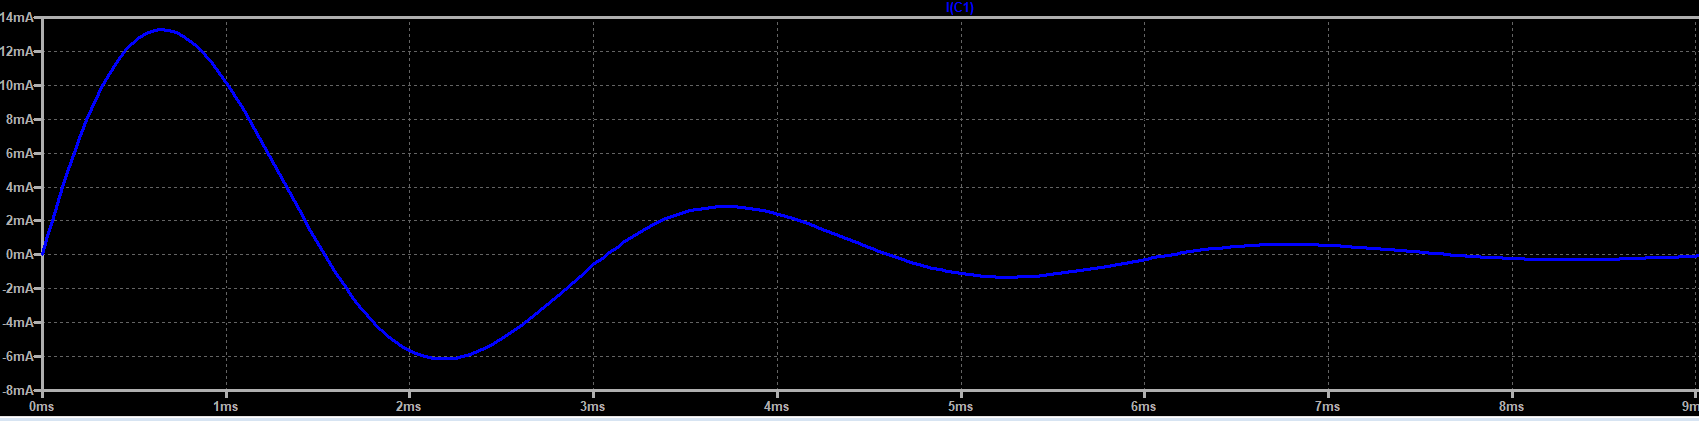
\includegraphics[scale=0.35]{carga-rlc-ic.PNG}
	\caption{La corriente del sistema.}
	\label{fig:-corrrlc}
\end{figure}

Luego, se obtuvo la gráfica de $v_c(t)$, y se la comparó con la obtenida mediante el uso del osciloscopio:
\flushleft
\begin{figure}[H]
	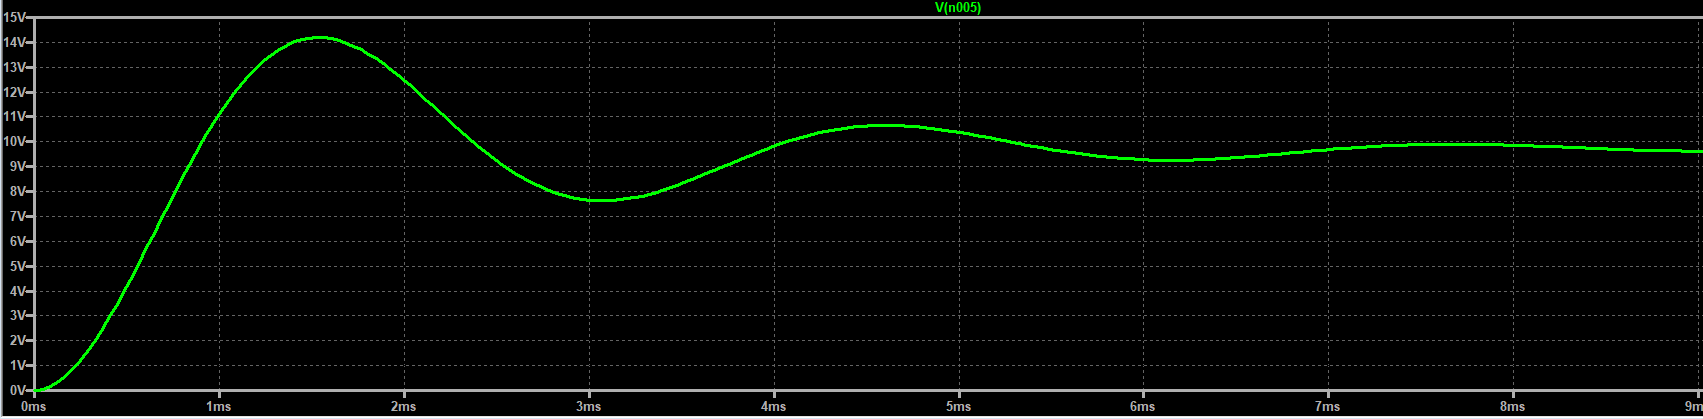
\includegraphics[scale=0.35]{carga-rlc-vc.PNG}
	\caption{Tension sobre el capacitor.}
	\label{fig:-tenrlc}
\end{figure}

Finalmente, se calcularon los intervalos de $R$ que hacen que el circuito sea subamortiguado, criticamente amortiguado y sobreamortiguado.

\[R_{sub}<1054 \Omega \quad R_{crit}= 1054 \Omega \quad R_{sobre}>1054 \Omega\]

\end{document}


